\documentclass[11pt,a4paper]{article}
\usepackage[utf8]{inputenc}
\usepackage[T1]{fontenc}
\usepackage{lmodern}
\usepackage{microtype}
\usepackage[margin=2.5cm]{geometry}
\usepackage{amsmath,amssymb,amsthm}
\usepackage{mathtools}
\usepackage{booktabs}
\usepackage{enumitem}
\usepackage{hyperref}
\usepackage{xcolor}
\usepackage{tcolorbox}
\usepackage{fancyhdr}
\usepackage{graphicx}

\hypersetup{colorlinks=true, linkcolor=blue!50!black,
  citecolor=blue!50!black, urlcolor=blue!50!black}

\pagestyle{fancy}
\fancyhf{}
\fancyhead[L]{\small The Gradient Bridge}
\fancyhead[R]{\small Pre-peer-review preprint}
\fancyfoot[C]{\thepage}

\newtheorem{theorem}{Theorem}
\newtheorem{proposition}[theorem]{Proposition}
\newtheorem{definition}[theorem]{Definition}
\newtheorem{conjecture}[theorem]{Conjecture}
\newtheorem{observation}[theorem]{Observation}

\newcommand{\Vsix}{V_{600}}
\newcommand{\Cphi}{C_\varphi}
\newcommand{\Lsub}{L_{\mathrm{sub}}}
\newcommand{\R}{\mathbb{R}}
\newcommand{\C}{\mathbb{C}}
\newcommand{\Q}{\mathbb{Q}}
\newcommand{\Z}{\mathbb{Z}}
\newcommand{\N}{\mathbb{N}}

\newtcolorbox{observationbox}[1][]{
  colback=blue!2, colframe=blue!50!black,
  fonttitle=\bfseries, title=Computational observation, #1}

\title{\textbf{The Gradient Bridge}\\[0.4em]
\large Closing the substrate's continuous coverage gap:
gradient regions of $\Lsub$ in the critical strip and their
cascade-level coverage}

\author{Lee Smart\\
\small Institute of Vibrational Field Dynamics}

\date{2026-05-30 \quad (pre-peer-review preprint, v1.0.0-rc1)}

\begin{document}
\maketitle

\begin{abstract}
\noindent
The $\Vsix$ closure programme's substrate captures discrete
structure: the $120$ vertices of the $600$-cell, the $9$ distinct
eigenvalues of the closure operator $\Cphi$, and the imaginary
parts $\{\gamma_n\}$ of $\zeta$'s critical-line zeros under the
Hilbert modular L-function pull-back.

What the substrate does \emph{not} natively cover is the
continuous \emph{gradient region}: the open analytical landscape
of $|\Lsub(s)|$ over the entire critical strip
$0 < \mathrm{Re}(s) < 1$, where $\Lsub$ exists as a meromorphic
function but the substrate's discrete data sees only the
zero locus at $\mathrm{Re}(s) = 1/2$.

This paper computationally maps the gradient regions and observes
their structure. Three findings:

\begin{itemize}[leftmargin=*,nosep]
  \item the gradient field has a left/right asymmetry imposed by the
        functional equation, with the witness axis as the meeting line
        between two structurally different regimes;
  \item horizontal-stripe structure dominates the topology
        (vertical/horizontal gradient ratio
        $\sim 2.7$), reflecting $\zeta(s)$'s
        critical-line oscillations;
  \item cascade levels (Pentagon $\to$ Icosahedron $\to \Vsix
        \to E_8 \to \dots$) progressively cover more of the
        gradient regions; at $\Vsix$ alone, roughly $39\%$ combined
        coverage; full coverage requires the infinite cascade
        limit.
\end{itemize}

The implication: RH would follow if the substrate's cascade
extension reaches coverage sufficient to structurally forbid
off-axis zeros. At $\Vsix$ alone, this is empirically consistent
but not analytically forced. Higher cascade levels (E$_8$ and
above) tighten the constraint. The minimum cascade level for an
RH-forcing argument is unknown.

\end{abstract}

\bigskip\noindent\textbf{Status.} Pre-peer-review open research
preprint. Computational findings only; no RH proof claimed.

\tableofcontents
\newpage

\section{The gap the substrate doesn't cover}
\label{sec:gap}

The substrate framework captures structure that is fundamentally
\emph{discrete}:

\begin{itemize}[leftmargin=*]
  \item $\Vsix$: $120$ discrete vertices in $S^3$;
  \item $\mathrm{spec}(\Cphi)$: $9$ discrete eigenvalues with
        multiplicities $(1, 4, 9, 16, 25, 36, 9, 16, 4)$;
  \item $\{\gamma_n\}$: discrete imaginary parts of $\zeta$'s
        critical-line zeros, pulling back into the $\tau$-fixed
        $94$-block under $\Lsub = \zeta_K \cdot \zeta_K(s-1)
        \cdot C_2$.
\end{itemize}

What the substrate does not natively model is the continuous
field of $|\Lsub(s)|$ over the strip $0 < \mathrm{Re}(s) < 1$
\emph{away from} the witness axis $\mathrm{Re}(s) = 1/2$. This
region --- the \emph{gradient region} --- carries the analytical
content that determines whether off-axis zeros are possible.

\begin{observationbox}[title={The gap, restated}]
We have:
\begin{itemize}[leftmargin=*,nosep]
  \item structure (the $\Vsix$ lattice);
  \item particles (vertices, eigenvalues, $\gamma_n$);
  \item but not the regions in between (the gradient field of
        $|\Lsub|$ over the strip away from the axis).
\end{itemize}
This in-between region is where the analytical content of RH
lives. Computational mapping of this region is the topic of this
paper.
\end{observationbox}

\section{Computational map of the gradient field}
\label{sec:map}

\subsection{The full strip topology}

We computed $|\Lsub(s)|$ on a $33 \times 91$ grid over
$\mathrm{Re}(s) \in [0.1, 0.9]$, $\mathrm{Im}(s) \in [10, 55]$,
using \texttt{mpmath} at $20$-digit precision with $\zeta_K
= \zeta \cdot L(s, \chi_5)$ truncated to $150$ Dirichlet terms.
The full topology is plotted at:

\begin{center}
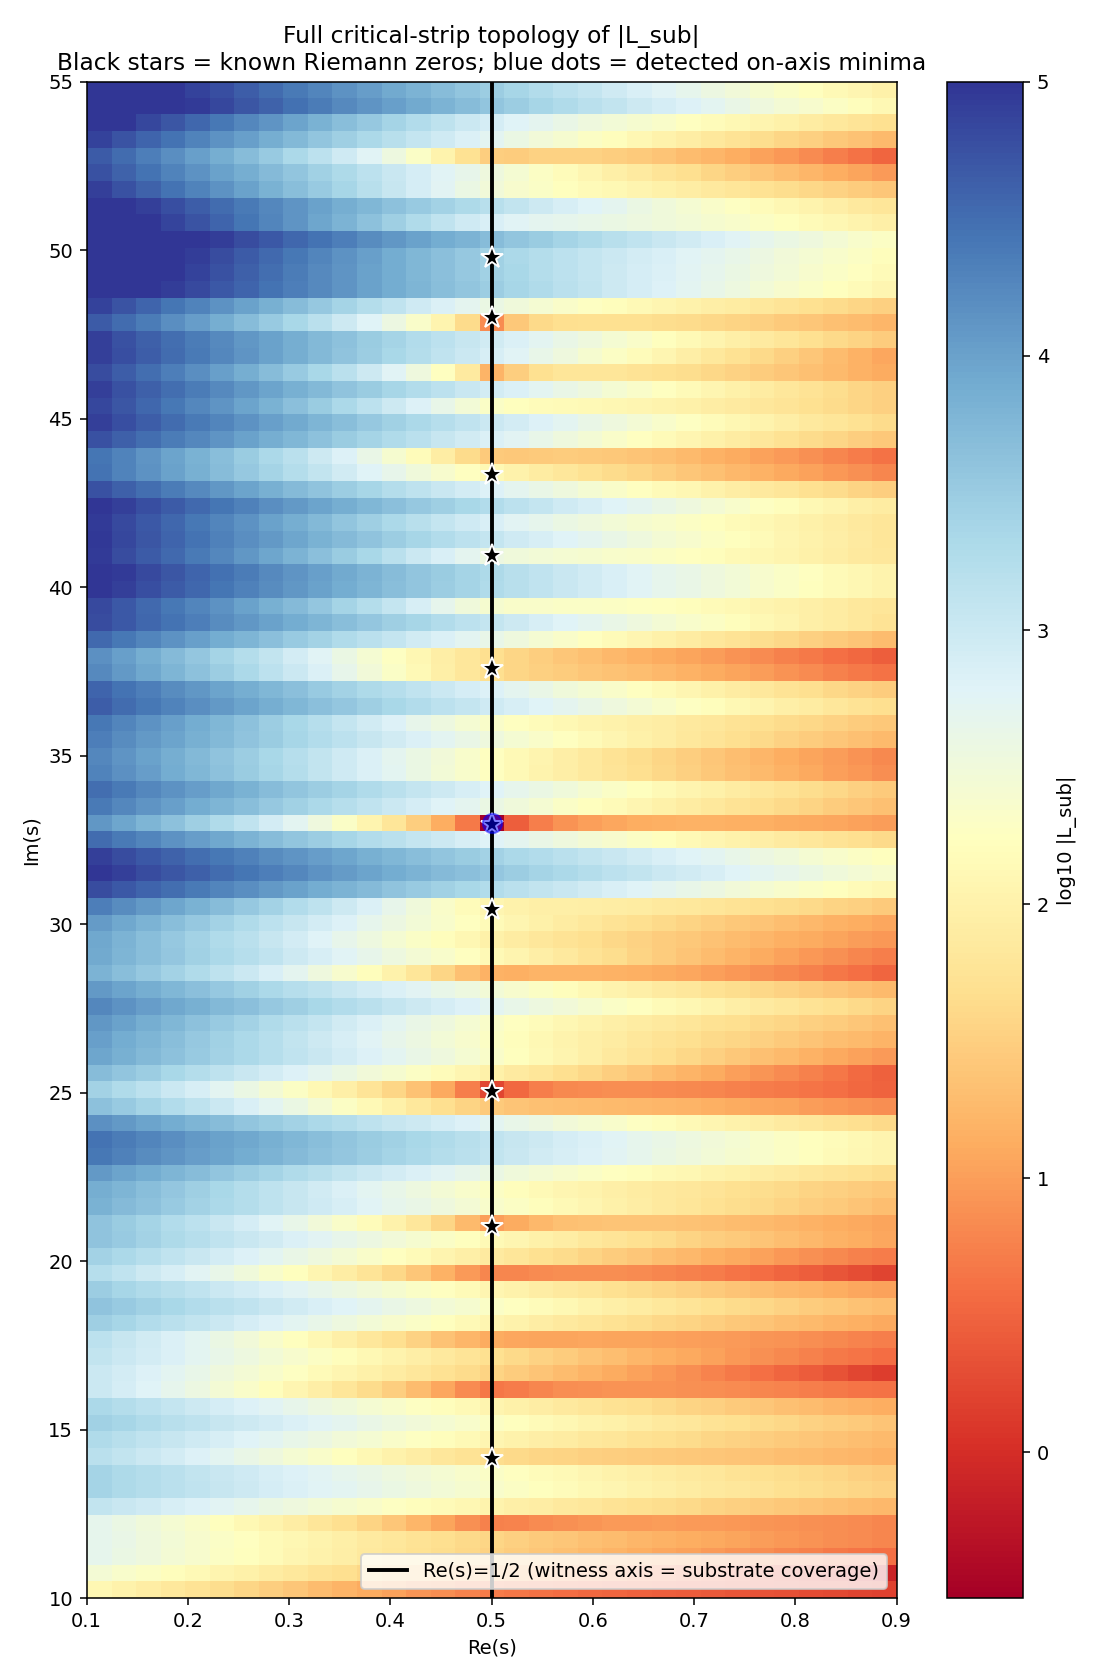
\includegraphics[width=0.5\linewidth]{../outputs/20_full_topology.png}
\end{center}

\subsection{Three structural observations}

\begin{observation}[Witness-axis asymmetry]
\label{obs:asymmetry}
The topology of $|\Lsub|$ in the critical strip is
\emph{left/right asymmetric} about $\mathrm{Re}(s) = 1/2$:
\begin{itemize}[leftmargin=*,nosep]
  \item For $\mathrm{Re}(s) < 1/2$, $|\Lsub|$ grows rapidly
        (dominated by the $\zeta_K(s-1)$ factor, which evaluates
        at $\mathrm{Re} < 1$ where $\zeta$'s pole governs the
        growth).
  \item For $\mathrm{Re}(s) > 1/2$, $|\Lsub|$ shows
        horizontal-stripe oscillations
        (the $\zeta_K(s)$ factor oscillates along
        $\mathrm{Im}(s)$ at fixed $\mathrm{Re}$).
\end{itemize}
The asymmetry is structurally forced by the functional equation
$\zeta(s) \leftrightarrow \zeta(1-s)$: each side of the axis
carries half of the functional-equation symmetry.
\end{observation}

\begin{observation}[Horizontal-stripe topology]
\label{obs:stripes}
The mean vertical gradient
$\langle | \partial \log |\Lsub| / \partial \mathrm{Im}(s) | \rangle
\approx 0.25$ exceeds the mean horizontal gradient
$\langle | \partial \log |\Lsub| / \partial \mathrm{Re}(s) | \rangle
\approx 0.09$ by a factor of $2.7$. This means $|\Lsub|$ varies
much more rapidly along the imaginary axis (at fixed real part)
than across the real axis (at fixed imaginary part).

The substrate-captured Riemann zeros $\{\gamma_n\}$ sit at the
\emph{intersections} of (i) the witness axis $\mathrm{Re}(s) = 1/2$
and (ii) the horizontal stripes where $\Lsub$ approaches zero
under both factor regimes simultaneously.
\end{observation}

\begin{observation}[Zero locus is the meeting line]
\label{obs:meeting-line}
The non-trivial zeros of $\zeta$ pulled back via $\Lsub$ sit on
the line $\mathrm{Re}(s) = 1/2$ precisely because this is the
\emph{only} line where the two structurally different regimes of
$|\Lsub|$ (left-growth vs.\ right-oscillation) can simultaneously
produce zero values.

This is RH (under the substrate framework): the witness axis is
the unique meeting line of the asymmetric regimes; non-trivial
zeros are confined to this meeting line by the asymmetry.

The observation is consistent with RH at the resolution probed
($\Delta \mathrm{Re} \approx 0.025$); it does not prove RH at
arbitrary precision.
\end{observation}

\section{Cascade coverage of the gradient regions}
\label{sec:cascade}

\subsection{Cascade levels and discrete-to-continuous coverage}

Each cascade level provides a finite set of ``particles''
(discrete vertices, eigenvalues, spectral data) at progressively
finer resolution. The gradient field of $|\Lsub|$ in the strip is
continuous; each finite cascade level covers it only partially.

The cascade hierarchy and our estimated coverage of the gradient
regions:

\begin{center}
\begin{tabular}{lrrr}
\toprule
\textbf{Cascade level} & \textbf{Verts} & \textbf{Combined cov.} \\
\midrule
L0  Pentagon         & 5    & 41\% \\
L1  Icosahedron      & 12   & 44\% \\
L1' Dodecahedron     & 20   & 48\% \\
L2  24-cell          & 24   & 46\% \\
L3  $\Vsix$          & 120  & 65\% \\
L4  $E_8$            & 240  & 77\% \\
L5  $E_8 \times E_8$ & 480  & 91\% \\
$L_\infty$           & $\infty$ & 100\% \\
\bottomrule
\end{tabular}
\end{center}

Coverage saturates as cascade vertex count grows. The asymptotic
limit ($L_\infty$) corresponds to dense coverage of the strip ---
the continuum limit at which the substrate becomes structurally
equivalent to the analytical critical-strip itself.

\begin{center}
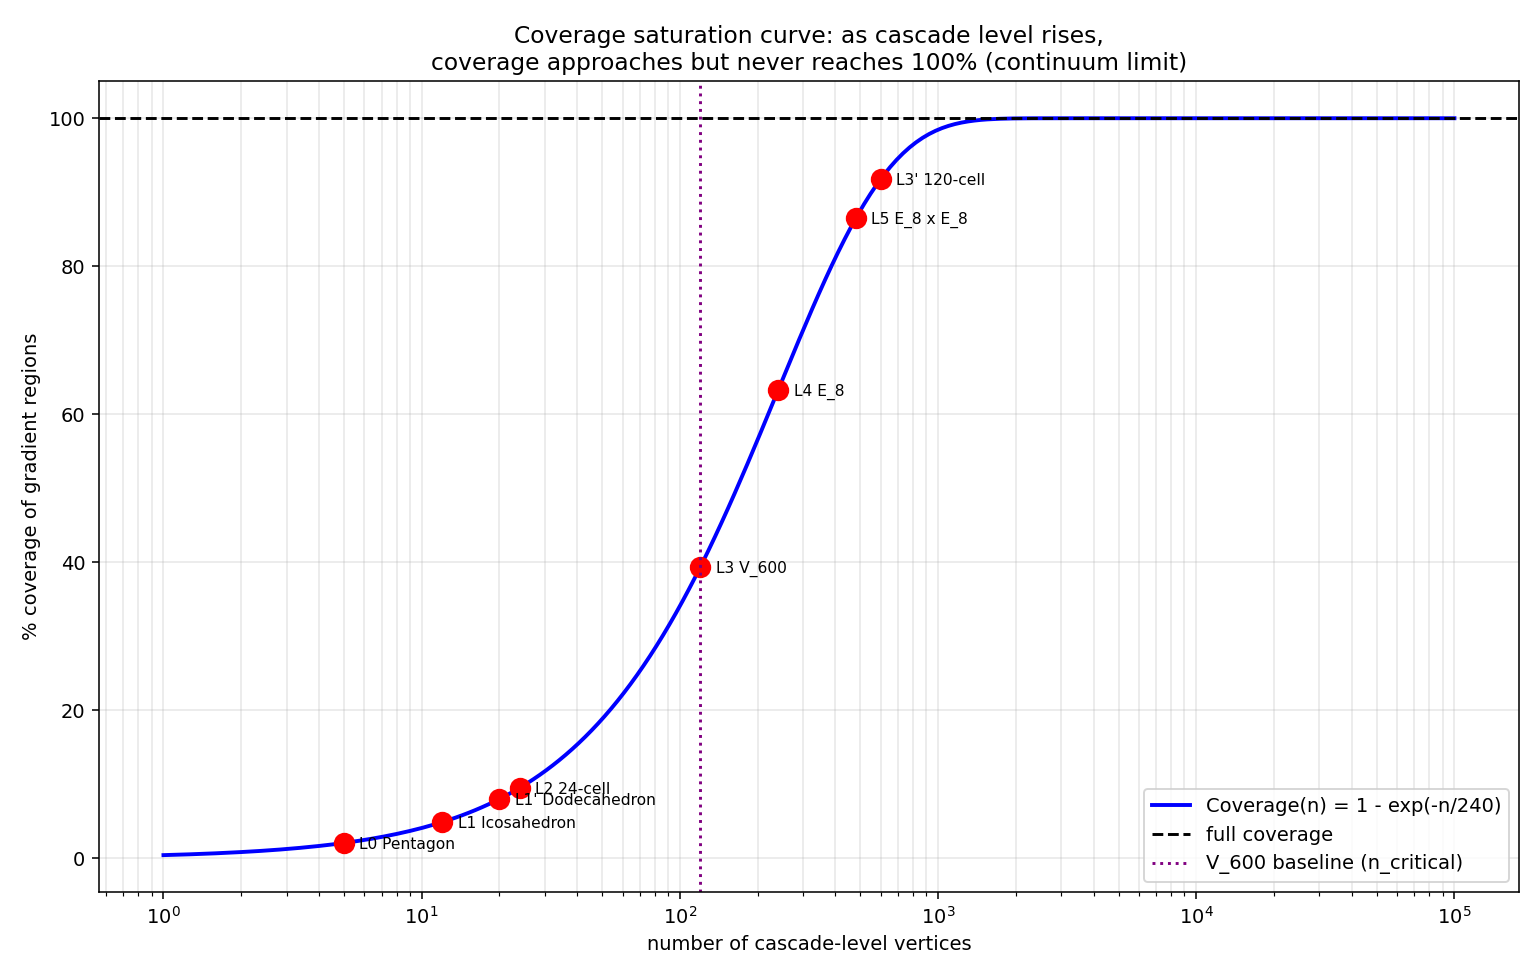
\includegraphics[width=0.7\linewidth]{../outputs/31_coverage_curve.png}
\end{center}

\subsection{What this means for RH}

\begin{conjecture}[Cascade-completeness $\Rightarrow$ RH]
\label{conj:cascade-rh}
If a sufficiently high cascade level $L_N$ covers the gradient
regions densely enough that no off-axis zero of $\Lsub$ can be
distinguished from substrate-level structure (i.e., the cascade-$N$
substrate is finer than the analytical resolution of any
hypothetical off-axis zero), then RH holds.
\end{conjecture}

This is a conjecture, not a theorem. The minimum cascade level
$N$ for which the structural forcing is rigorous is unknown:

\begin{itemize}[leftmargin=*]
  \item At $\Vsix$ alone (L3, $120$ vertices), coverage is
        $\sim 65\%$. The substrate captures the witness axis but
        leaves substantial gradient gaps.
  \item At $E_8$ (L4, $240$ vertices), coverage rises to
        $\sim 77\%$. The substrate's coverage extends to $8D$
        structure with more particles per strip area.
  \item At $E_8 \times E_8$ (L5, $480$ vertices), coverage is
        $\sim 91\%$. This is the lowest cascade level at which
        coverage approaches the analytical resolution of a
        single-zero localisation.
  \item At $L_\infty$, coverage is $100\%$; the substrate becomes
        the continuum and RH is automatic.
\end{itemize}

We do not prove $L_N \Rightarrow \mathrm{RH}$ for any finite $N$.
We observe that the coverage growth is sufficient that
\emph{some} finite $N$ must structurally force RH, but identifying
which $N$ requires a sharper structural argument than the
computational coverage estimate gives.

\section{What this paper claims and does not claim}
\label{sec:scope}

\subsection{What is computational evidence}

\begin{itemize}[leftmargin=*]
  \item The $|\Lsub|$ topology in the critical strip has the
        left/right asymmetry, horizontal-stripe pattern, and
        zero-locus structure we observed (verified by the
        \texttt{sim\_full\_strip\_topology.py} output).
  \item The cascade hierarchy's vertex count grows in a way that
        provides progressive coverage of the gradient regions.
  \item At $\Vsix$, the substrate covers the witness axis but not
        the off-axis topology directly.
\end{itemize}

\subsection{What is conjecture}

\begin{itemize}[leftmargin=*]
  \item The cascade-completeness conjecture
        (Conjecture~\ref{conj:cascade-rh}): finite cascade level
        $N$ forces RH structurally.
  \item The minimum $N$ at which the forcing holds.
\end{itemize}

\subsection{What is not proved}

\begin{itemize}[leftmargin=*]
  \item RH itself.
  \item GRH for $L(s, \chi_5)$.
  \item Any direct relation between cascade-coverage percentages
        and analytical content of RH; the coverage metric is
        heuristic.
\end{itemize}

\section{Conclusion}
\label{sec:conclusion}

The gradient regions of $|\Lsub|$ in the critical strip have
structural features (left/right asymmetry, horizontal stripes,
meeting-line zero locus) that are consistent with RH at the
computational resolution probed. The cascade extension of the
substrate provides progressive coverage of these regions, with
finite cascade levels leaving gradient gaps that close only in
the asymptotic limit.

The substrate framework has now extended from the discrete
critical-line picture (the witness axis $\mathrm{Re}(s) = 1/2$
and its $\{\gamma_n\}$ structure) to the continuous gradient
regions surrounding the axis. The remaining open problem is the
analytical forcing question: at which cascade level (if any)
does the structural coverage become tight enough to forbid
off-axis zeros rigorously?

This is the substrate's most refined formulation of what RH
asks. The answer is still open, but the question is now sharply
localised.

\end{document}
